\documentclass[border=0.5mm]{standalone}
\usepackage{tikz}
\usetikzlibrary{arrows.meta, positioning}

\begin{document}

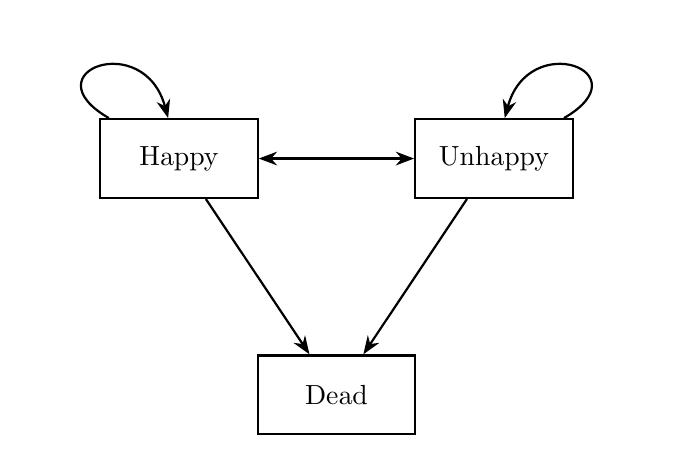
\begin{tikzpicture}[
    % Define node style
    node style/.style={
        draw, % Draw border
        rectangle, % Rectangle shape
        minimum width=2cm, % Minimum width
        minimum height=1cm, % Minimum height
        align=center % Center alignment
      },
    % Define arrow style
    ->, % Default arrow direction
    >=Stealth, % Arrow type
    thick % Line thickness
  ]

  % Define nodes
  \node[node style] (Happy) at (-2, 0) {Happy}; % Node h on the left, height at 0
  \node[node style] (Unhappy) at (2, 0) {Unhappy};  % Node u on the right, height at 0, same level as h
  \node[node style] (Dead) at (0, -3) {Dead}; % Node d at the bottom, below the middle of h and u

  % Draw arrows and labels
  % p_hh: self-loop arrow, keep curved
  \draw[->] (Happy) to[out=150, in=105, looseness=4] (Happy);

  % Bidirectional arrow between Happy and Unhappy
  \draw[<->] (Happy) -- (Unhappy);

  % p_uu: self-loop arrow, keep curved
  \draw[->] (Unhappy) to[out=30, in=75, looseness=4] (Unhappy);

  % p_hd: from h to d, straight
  \draw[->] (Happy) -- (Dead);

  % p_ud: from u to d, straight
  \draw[->] (Unhappy) -- (Dead);

\end{tikzpicture}

\end{document}
